\documentclass[../main.tex]{subfiles}
\begin{document}
\chapter{O CONJUNTO DOS NÚMEROS NATURAIS E OS AXIOMAS DE PEANO}\label{cap-naturais}
 
Neste capítulo apresentaremos a formalização aritmética do conjunto dos números naturais. Primeiro será apresentada uma breve parte histórica e, após isso, enunciaremos os axiomas de Peano. Depois definiremos uma adição, uma multiplicação e uma relação de ordem, bem como listaremos algumas propriedades básicas e faremos suas demonstrações. As referências básicas desse capítulo são \textcite{domingues-2009} e \textcite{ferreira}.

\section{Um pouco de história}

Uma possível narrativa para o início do trabalho com números seria a necessidade de pastores efetuarem a contagem de animais em seus rebanhos, embora essa narrativa não seja definitiva \Cite{roque}. Essa iniciação com números e o conhecimento obtido pode ter encontrado dois caminhos (ou fins) possíveis, foram mantidos ao longo do tempo ou não. Nesse sentido não é possível estabelecer uma matemática definitiva e uma única evolução \Cite[p. 35]{roque}. 

Ao longo da históra, foram desenvolvidos muitos conjuntos numéricos, para resolver problemas em que os conjuntos anteriores não eram adequados ou suficientes. 
Com o avanço da matemática, acabou-se esbarrando em problemas que as crenças e técnicas da época não conseguiam resolver, assim uma formalização era necessária, mesmo que esse não fosse o objetivo principal, mas sim resolver esses problemas \Cite[p. 407]{roque}.

Quem fundamentou a aritmética como conhecemos hoje foi o italiano Giuseppe Peano (1858 - 1932), mas houve tentativas anteriores, em que podemos citar Frege (1848-1925). 
Peano conseguiu, entre outros fatores, usar boas escolhas para símbolos, muitos dos quais usamos atualmente, e também por causa da explicitação das regras por meio de símbolos e a ausência de hipóteses ocultas \Cite[p. 415]{boyer}

O trabalho de Peano ficou conhecido como Axiomas de Peano. Ele fundamentou a sua aritmética com 9 axiomas e 3 conceitos primitivos, como está apresentado na \Cref{fig:axiomas-peano}.

\begin{figure}
    \begin{center}
        \caption{A versão original dos axiomas de Peano}\label{fig:axiomas-peano}
        \hbox{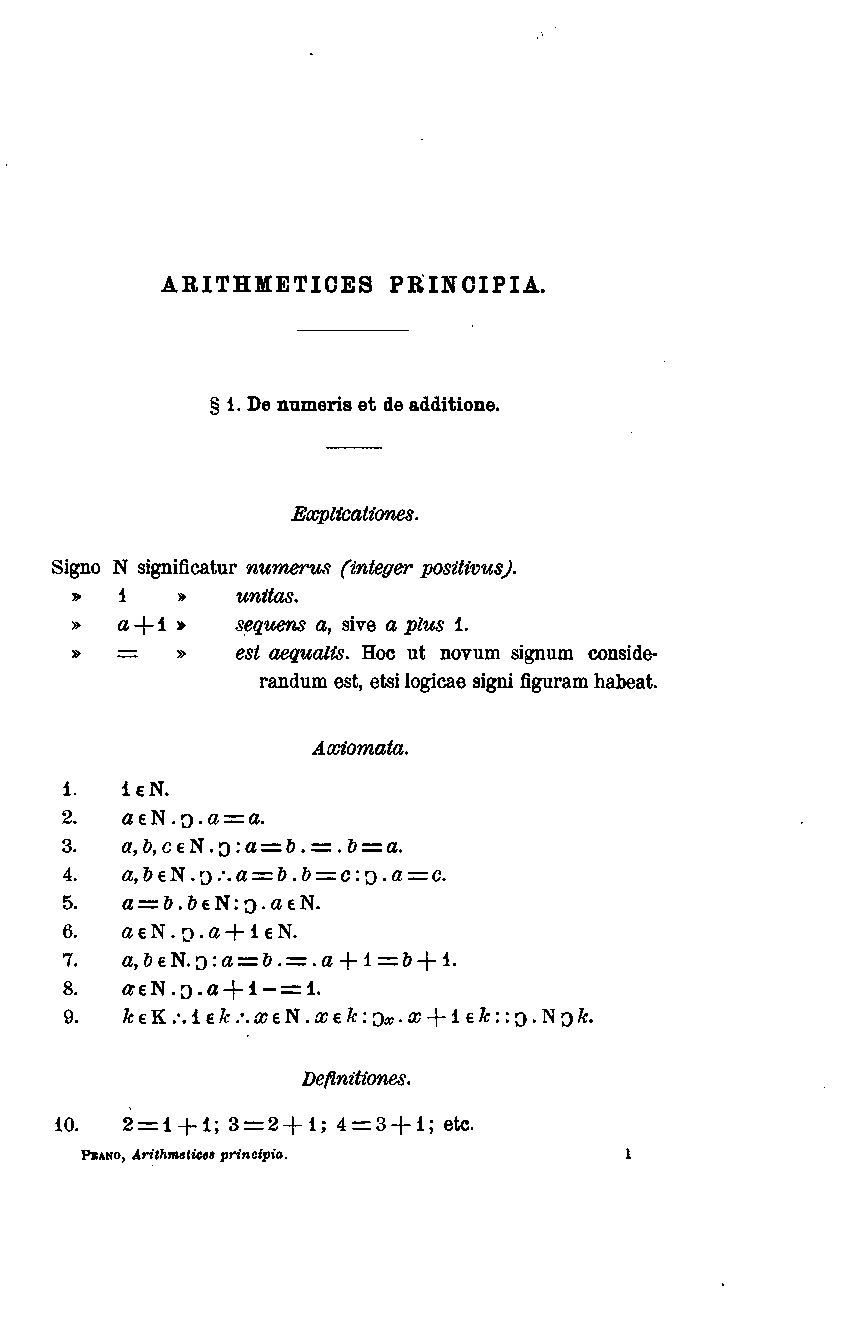
\includegraphics[scale=1]{../include/peano_axioms_original}}
        % \caption{Fonte: Archive.org\footnote{Disponível em <\url{https://ia903400.us.archive.org/12/items/arithmeticespri00peangoog/arithmeticespri00peangoog.pdf}>. Acesso em: 05 jun. 2023}; Giuseppe Peano (1889)}
        Fonte: Archive.org; Giuseppe Peano (1889)
       % \footnote{Disponível em <\url{https://ia903400.us.archive.org/12/items/arithmeticespri00peangoog/arithmeticespri00peangoog.pdf}>. Acesso em: 05 jun. 2023}
    \end{center}  
\end{figure}

Antes de continuarmos, podemos recolocar uma analogia da matemática com um jogo:

\begin{displayquote} Ao criar um jogo, é importante que suas regras sejam suficientes e consistentes. Por \emph{suficiente} queremos dizer que as regras devem estabelecer o que é permitido fazer em qualquer situação que possa vir a ocorrer no desenrolar de uma partida do jogo. Por \emph{consistente} queremos dizer que as regras não devem contradizer-se, ou sua aplicação levar a situações contraditórias \Parencite[p. 13-14]{barbosa}.
\end{displayquote}

Para nós, as peças do jogo serão o conceito de um, o conceito de número natural, e o conceito da relação sucessor. As regras do jogo serão os axiomas que relacionarão esses três conceitos primitivos. Nessa analogia, as peças não são muito importantes, mas as regras o serão.

\section{Axiomas de Peano}
O nosso estudo dos números naturais será iniciado pela apresentação dos axiomas de Peano, que relacionam os conceitos primitivos adotados. Serão apresentados 5 axiomas ao invés de 9 porque assumimos a teoria de conjuntos e a lógica elementar como fundamental, assim dispomos de uma relação de igualdade '$=$' que é reflexiva, simétrica e transitiva. Peano colocou essas propriedades da igualdade como axiomas, o que não precisamos fazer aqui. Na verdade, pode-se até optar por versões mais reduzidas desse conjunto de axiomas, podemos citar \textcite{ferreira} e \textcite{lima-analise-1}, em que ambos utilizam 3 axiomas.

\begin{axi}\label{nat-axi-existeConjuntoNeFuncaoS}
    Existe um conjunto de exatamente todos os números naturais, que será denotado por $\mathbb{N}$, e existe uma função $s: \mathbb{N} \rightarrow \mathbb{N}$, que é a relação "sucessor". 
\end{axi}
\begin{axi}\label{nat-axi-umNatural}
    Um é um número natural, isto é, $1 \in \mathbb{N}$.
\end{axi}
\begin{axi}\label{nat-axi-umNaoSucessor}
    Um não é sucessor de nenhum número, isto é, $1 \not \in Im(s)$ ou ainda, $\not \exists a \in \mathbb{N} : s(a) = 1$.
\end{axi}
\begin{axi}\label{nat-axi-SInjetora}
    $s$ é injetora, isto é, $s(a) = s(b) \implies a = b$ \footnote{Vale notar a contra-positiva que estabelece, nesse caso: $a \neq b \implies s(a) \neq s(b)$.}.
\end{axi}
\begin{axi}\label{nat-axi-inducaoFinita}
    Seja $\mathbb{S}$ um subconjunto de $\mathbb{N}$. Caso $1 \in \mathbb{S}$ e se, para todo $k$ em $\mathbb{S}$, ocorrer que $s(k)$ também esteja em $\mathbb{S}$, então $\mathbb{S} = \mathbb{N}$. Isso é o mesmo que colocar: \\
     \[ \mathbb{S} \subseteq \mathbb{N} \land 1 \in \mathbb{S} \land ( k \in \mathbb{S} \Rightarrow s(k) \in \mathbb{S}) \implies \mathbb{S} = \mathbb{N} .\]
\end{axi}
Este último axioma é chamado de axioma da indução finita.

Conforme os axiomas apresentados, deve ser notado que o conjunto $\mathbb{N}$ (na nossa axiomatização) não tem o $0$ (zero) que é, usualmente, o neutro da soma em $\mathbb{N}$. O intuito de construir $\mathbb{N}$ a partir do $1$ é pela questão que às vezes surge em diversas situações: "$0$ é um número natural?". Em especial, o próprio \textcite{lima-site} diz que o zero pode ser ou pode não ser um número natural. É dito que fica a critério de conveniência, embora para nós, seja 'inconveniente' perder o neutro da soma (que aparecerá sua primeira vez em $\mathbb{Z}$). 

Justificamos essa escolha pois a ausência do zero terá algumas consequências e exigirá alguns ajustes, que poderão ser observados na nossa construção. Além disso, a bibliografia principal trata o zero como um número natural, então a construção será necessariamente com essas adaptações, o que, em nossa visão, é algo positivo para o desenvolvimento do trabalho, apesar do resultado final, em certo ponto de vista, ficar prejudicado pela ausência do $0$.

%% ISSO AQUI SE CHAMA REMENDO -> É UM REMENDO ->> REMENDDDDDDDOOOOOO

Observemos também que o próprio Peano começou sua teoria originalmente pelo $1$ e, somente em trabalho posterior, colocou o $0$ como o primeiro número natural.

Para comerçarmos nosso desenvolvimento, podemos notar que o \Cref{nat-axi-umNatural} garante que $\mathbb{N} \neq \emptyset $. Além disso, o \Cref{nat-axi-existeConjuntoNeFuncaoS} garante que $s(1) \in \mathbb{N}$, também $s(s(1)) \in \mathbb{N}$, $s(s(1)) \in \mathbb{N}$ e assim por diante.

Em seguida, apresentamos um lema que será necessário para a ampliação de nosso ferramental inicial.
\begin{lema}\label{nat-lema-nenhumNumeroProprioSucessor}
    Nenhum número natural é seu próprio sucessor, ou seja, $a \in \mathbb{N} \implies a \neq s(a) $.
\end{lema}
\begin{dem}
    Faremos por indução.\\
    Seja $\mathbb{S} = \{a \in \mathbb{N} : a \neq s(a) \}$.
    Os axiomas \ref{nat-axi-umNatural} e \ref{nat-axi-umNaoSucessor} garantem que $1 \in \mathbb{S}$.\\
    Supondo que $ k \in \mathbb{S}$, onde $ k \neq s(k)$, vamos provar que o sucessor de $k$ é diferente do sucessor do sucessor de $k$, isto é, $s(k) \neq s(s(k))$. Como $k \neq s(k)$ e $s$ é injetora pela contrapositiva do \Cref{nat-axi-SInjetora}, concluímos que $s(k) \neq s(s(k))$. Pelo \Cref{nat-axi-inducaoFinita}, conclui-se que $\mathbb{S} = \mathbb{N}$ e, portanto, para qualquer natural $a$ tem-se que $a \neq s(a)$.
\end{dem}
\begin{teo}\label{nat-teo-todoNaturalESucessor}
    Todo número natural, exceto o $1$, é sucessor de algum outro número natural, que é único.
    % , isto é, $\forall x (x \in \mathbb{N} \land x \neq 1 \implies \exists! y : s(y) = x)$.
\end{teo}
\begin{dem}
    A prova é feita por indução.  \\ 
    Seja $\mathbb{S} = \{x \in \mathbb{N} : x \neq 1 \implies (\exists y \in \mathbb{N} \land s(y) = x) \}$.\\
    Sabemos que $1 \in \mathbb{S}$ porque $x = 1$ torna o antecedente falso, assim a implicação é logicamente verdadeira. Suponhamos $k \in \mathbb{S}$. Assim, $k$ é o sucessor de algum $y \in \mathbb{N}$, ou seja, $k = s(y)$. É imediato que $s(k)$ é sucessor de $k \in \mathbb{N}$, e portanto $s(k) \in \mathbb{S}$. Pelo \Cref{nat-axi-inducaoFinita} concluímos que $\mathbb{S}$ = $\mathbb{N}$, ou seja, todo número natural diferente de $1$ é sucessor de algum número natural.

    Além disso, fixado um $k \in \mathbb{N}$ com $k \neq 1$, o elemento $y \in \mathbb{N}$ tal que $s(y) = k$ é único. De fato, se $x,y$ são naturais tais que $s(x) = s(y) = k$, pelo \Cref{nat-axi-SInjetora} obtemos que $x = y$.
\end{dem}
\begin{obs}
    Diremos que o número $y$ do teorema anterior é o antecessor de $x = s(y)$. Além disso vale notar que $s$ (conforme definida no \Cref{nat-axi-existeConjuntoNeFuncaoS}) não é sobrejetora somente pelo fato de seu contradomínio ser $\mathbb{N}$. Mas se considerarmos o caso restrito para $\mathbb{N} \setminus \{1\}$, teremos que $s$ é uma bijeção.
\end{obs}

Utilizaremos a notação usual para os números naturais, isto é, $\mathbb{N} = \{ 1, 2, 3, 4, ...\}$, onde $2 \defeq s(1), 3 \defeq s(2), 4 \defeq s(3)$ e assim por diante.

%%% ADICAO %%%


\section{A adição em $\mathbb{N}$}
A adição em $\mathbb{N}$ é a operação que mais intuitivamente está relacionada com a contagem e união de coisas discretas.
\begin{defi}\label{nat-def-soma}
Sejam $a, b \in \mathbb{N}$. A adição entre $a$ e $b$, denotada por $a + b$ é definida com as seguintes condições: 
    \begin{enumerate}[label=(\roman*)]
        \item\label{nat-dummySomaMaisUm} $a + 1 = s(a)$;
        \item\label{nat-dummySomaMaisQualquer} $a + s(b) = s(a+b)$.
    \end{enumerate}
\end{defi}
A ideia por trás desta definição de adição é a de recursão. Nesse caso o item \ref{nat-dummySomaMaisUm} nos diz como somar qualquer número natural com o $1$. O item \ref{nat-dummySomaMaisQualquer} nos diz como somar um elemento qualquer com o sucessor de outro, só que pelo \Cref{nat-teo-todoNaturalESucessor} todo natural diferente de $1$ é sucessor de alguém.
\begin{ex}
    Podemos somar $2 + 3$ do seguinte modo:
    \[ 2+3 = 2+s(2) = s(2+2) = s(2+s(1)) = s(s(2+1))) = s(s(s(2))) = s(s(3))=s(4)=5. \]
\end{ex}

\begin{teo}
    A adição dada pela \Cref{nat-def-soma} é uma função, que associa uma dupla de números naturais em um único número natural.
\end{teo}
\begin{dem}
    A prova de que a soma está bem definida para quaisquer $a,b \in \mathbb{N}$ é dada a seguir:
    Dado $a \in \mathbb{N}$ fixo, seja $\mathbb{S} = \{ x \in \mathbb{N} : a + x \ \text{está definido} \}$. Temos que $a + 1 = s(a)$ está definido, portanto $1$ está em $\mathbb{S}$. 
    Agora consideremos um dado $k \in \mathbb{N}$, em que $a+k$ esteja bem definida. Temos então que $a + s(k) = s(a+k)$, como $a+k$ está definido, o sucessor também está definido, pelo \Cref{nat-axi-inducaoFinita}, temos que $\mathbb{S} = \mathbb{N}$.
\end{dem}
\begin{lema}\label{nat-lema-somaUmComuta}
    O $1$ comuta com qualquer número na soma, isto é, $ \forall x \in \mathbb{N}, x + 1 = 1 + x$.
\end{lema}
%       Template
%        Seja $\mathbb{S} = \{ x \in \mathbb{N} : \}$
\begin{dem}
    Seja $\mathbb{S} = \{ x \in \mathbb{N} : x + 1 = 1 + x\}$. O $1$ está em $\mathbb{S}$ pois $1 + 1 = 1 + 1$.
    Supondo $k \in \mathbb{S}$, temos que $k+1 = 1+k$. Queremos provar que $s(k)$ também está em $\mathbb{S}$. Como
    $s(k) + 1 = s(s(k)) = s(k+1) = s(1+k) = 1 + s(k)$. Portanto $s(k)$ também está em $\mathbb{S}$ sempre que $k$ também está, o que pelo \Cref{nat-axi-inducaoFinita}, $\mathbb{S} = \mathbb{N}$.
\end{dem} \\

\begin{prop}\label{nat-teo-somaPropriedades}
    A adição no conjunto dos números naturais tem as seguintes propriedades:
    \begin{enumerate}[label=(\roman*)]
        \item Fechamento;
    	\item Associativa;
    	\item Comutativa;
        \item Lei do cancelamento;
        \item Se $a,b \in \mathbb{N}$, então $a + b \neq a$;\label{nat-teo-AmaisBdiffA}
    	\item Inexistência de neutro: $\not\exists \mathfrak{e} \in \mathbb{N} : \forall a, a + \mathfrak{e} = \mathfrak{e} + a = a$.
    \end{enumerate}
\end{prop}

\begin{dem}
    Antes de demonstrarmos propriamente, façamos a suposição que $a,b,c \in \mathbb{N}$ são números fixados.
    \begin{enumerate}[label=(\roman*)]    
        \item Fechamento: \\
            Seja $\mathbb{S} = \{ x \in \mathbb{N} : a + x \in \mathbb{N} \}$. Obviamente o $1$ está em $\mathbb{S}$. Suponhamos então que $k \in \mathbb{S}$, queremos  garantir que $s(k) \in \mathbb{S}$. Temos então que $a + k \in \mathbb{N}$ o que implica que $a + s(k) = s(a + k) \in \mathbb{N}$, pois pelo \Cref{nat-axi-existeConjuntoNeFuncaoS}, a função $s$ tem contradomínio $\mathbb{N}$. Como $s(k) \in \mathbb{S}$, pelo \Cref{nat-axi-inducaoFinita} concluímos que $\mathbb{S} = \mathbb{N}$.
        \item Associativa: \\
             Seja $\mathbb{S} = \{ x \in \mathbb{N} : (a + b) + x = a + (b + x) \}$. Temos que \\
             $(a + b) + 1 = s(a + b) = a + s(b) = a + (b + 1)$, o que mostra que o $1$ está em $\mathbb{S}$. 
             Mostraremos que $k \in \mathbb{S} \implies s(k) \in \mathbb{S}$. De fato, supondo que $(a+b)+k = a+(b+k)$, temos:
             \[ (a + b) + s(k) = s( (a + b) + k) = s(a + (b + k)) = a + s(b + k) = a + (b + s(k)). \] 
             Pelo \Cref{nat-axi-inducaoFinita} concluímos que $\mathbb{S} = \mathbb{N}$.
        \item Comutativa: \\
            Consideremos o conjunto $\mathbb{S} = \{ x \in \mathbb{N} : a + x = x + a\}$. O $1 \in \mathbb{S}$ pois 
            $a + 1 = 1 + a$ conforme o \Cref{nat-lema-somaUmComuta}.
            Provemos então que, se $k \in \mathbb{S}$, então $s(k) \in \mathbb{S}$. De fato, supondo $a+k = k+a$ temos que 
            \[ a + s(k) = s(a + k) = s(k + a) = k + s(a) = k + (a + 1) = (k + 1) + a = s(k) + a. \]
            Pelo \Cref{nat-axi-inducaoFinita} concluímos que $\mathbb{S} = \mathbb{N}$.
        \item Lei do cancelamento:  \\
            Seja $\mathbb{S} = \{ x \in \mathbb{N} : x + b = x + c \implies b = c \}$, vamos provar que $\mathbb{S}$ = $\mathbb{N}$. Obviamente o $1$ está em $\mathbb{S}$ pois $1 + b = 1 + c \iff s(b) = s(c)$ e pelo \Cref{nat-axi-SInjetora}, se dois elementos tem sucessores iguais, eles próprios são iguais. Suponha $k + b = k + c \implies b = c$, temos que
            \begin{align*}
                s(k) + b = s(k) + c &\implies (k+1)+b = (k+1)+c \\
                &\implies (k + b) + 1 = (k + c) + 1 \\
                &\implies s(k+b) = s(k+c) \text{(pelo \Cref{nat-axi-SInjetora})}\\
                &\implies k+b = k+c. 
            \end{align*}
            A hipótese de indução garante que $b = c$. Desse modo, $s(k) \in \mathbb{S}$ e, pelo \Cref{nat-axi-inducaoFinita} concluímos que $\mathbb{S} = \mathbb{N}$. 
        \item $a + b \neq a$;\\
            A demonstração consiste em usar o \Cref{nat-teo-todoNaturalESucessor}, pois sabemos que um número natural ou é igual a $1$, ou é sucessor de algum outro número natural e no final obter que $1$ é sucessor de algum número natural, contrariando o \Cref{nat-axi-umNaoSucessor}. Assim, consideremos quatro casos para $a$ e $b$, sendo iguais a $1$ ou diferente de $1$ (que são todas as combinações possíveis), supondo que $a+b=a$, e mostraremos que todos são absurdos:
            \begin{enumerate}[label=(\arabic*)]
            \item $a=1 \land b=1$: \\
                Temos $a+b=a \iff 1+1=1$, o que é absurdo. 
            \item $a=s(x) \land b=1$, para algum $x \in \mathbb{N}$: \\
                Temos $a+b=a \iff s(x) + 1 = s(x) \iff s(s(x)) = s(x)$, o que é absurdo. 
            \item $a=1 \land b=s(y)$, para algum $y \in \mathbb{N}$: \\
                Temos $a+b=a \iff 1+ s(y) = 1 \iff s(1+y) = 1$, o que é absurdo. 
            \item $a=s(x) \land b=s(y)$, para algum $x \in \mathbb{N}$ e algum $y \in \mathbb{N}$: \\
                Temos 
                \[ a+b=a \iff s(x) + s(y) = s(x) \iff x + 1 + y + 1 = x + 1 \iff s(1 + y) = 1, \]
                o que é absurdo.
            \end{enumerate}
    
        \item Inexistência de neutro: \\
            Como consequência da demonstração anterior, não existe neutro na adição no nosso conjunto de números naturais, isto é, não existe $\mathfrak{e} \in \mathbb{N}$ tal que para qualquer $a \in \mathbb{N}$, vale $a + \mathfrak{e} = \mathfrak{e} + a = a$.
    \end{enumerate}
\end{dem}
 
% Podemos observar que como não existe neutro, não poderemos aplicar descuidadamente as outras propriedades, por exemplo: não poderíamos ter provado que $a \neq a + 1 $ usando a lei do corte e supondo que fossem iguais, assim: $a = a+ 1 \implies 0 = 1$, porque isso não faz sentido no nosso desenvolvimento. Também podemos observar que a lei do cancelamento é independente da \Cref{agb-teo-leiCancelamento}, uma vez que não temos neutro.

% %%% MULTIPLICACAO %%%
% A multiplicação toma seu lugar como uma operação de redução da soma. Essa ideia de notação resumida pode ser explorada quando se faz o uso do sistema posicional, mas não faremos o uso do sistema posicional. 

\section{A multiplicação em $\mathbb{N}$}
\begin{defi}\label{nat-def-produto}
    Sejam $a, b \in \mathbb{N}$. A multiplicação entre $a$ e $b$, denotada por $a \cdot b$ é definida com a as seguintes condições: 
	\begin{enumerate}[label=(\roman*)]
		\item $a \cdot 1 = a$;
		\item $a \cdot s(b) = a \cdot b + a$.
	\end{enumerate}
\end{defi}

\begin{teo}
    Para a multiplicação de números naturais são válidas as seguintes propriedades:
    \begin{enumerate}[label=(\roman*)]
        \item Fechamento;
        \item Da existência do elemento neutro; 
        \item Distributiva;
        \item Comutativa;
        \item Associativa;
        \item Para $a,b \in \mathbb{N}$ ocorre que, $a \cdot b = 1 \implies a = b = 1$.
    \end{enumerate}
\end{teo}
% template
% Seja $\mathbb{S} = \{ x \in \mathbb{N} : \}$
\begin{dem}
    Antes de demonstrarmos propriamente, façamos a suposição que $a,b,c \in \mathbb{N}$ são números fixos. Provaremos por indução, exceto no último item.
    \begin{enumerate}[label=(\roman*)]
        \item Fechamento: \\
            Seja $\mathbb{S} = \{x \in \mathbb{N} : a \cdot x \in \mathbb{N} \}$.
            O $1$ está em $\mathbb{S}$ pois $1 \cdot 1 = 1$. Supondo que é válido $ak \in \mathbb{N}$ para algum $k \in \mathbb{N}$, temos $a \cdot s(k) = ak + a$. Como tanto $ak$ quanto $a$ são números naturais, e como a soma é fechada em $\mathbb{N}$, temos que $ak + a \in \mathbb{N}$. Pelo \Cref{nat-axi-inducaoFinita}, $\mathbb{S}$ = $\mathbb{N}$. 
        \item Da Existência do elemento neutro: \\
            Seja $\mathbb{S} = \{ x \in \mathbb{N} : 1 \cdot x = x \cdot 1  = x \}$. O $1$ está em $\mathbb{S}$ pois $1 \cdot 1 = 1 \cdot 1 = 1$. Supondo que $k \in \mathbb{S}$ vamos concluir que $s(k) \in \mathbb{S}$.
            De fato, supondo $1 \cdot k = k \cdot 1$ temos que
            \[ 1 \cdot s(k) = 1 \cdot k + 1 = k \cdot 1 + 1 = k + 1 = s(k) = s(k) \cdot 1. \] 
            Pelo \Cref{nat-axi-inducaoFinita}, $\mathbb{S} = \mathbb{N}$.
            
            % \\ Além disso, sejam $e_1, e_2$ dois elementos neutros. Então $e_1 = e_1 \cdot e_2 = e_2 \implies e_1 = e_2$, portanto o neutro é único. Além disso a definição de multiplicação nos diz que é o $1$ quem é o neutro. 
        \item Distributiva à direita: 
            Seja $\mathbb{S} = \{ x \in \mathbb{N} : ( a + b ) x = ax + bx \}$. Temos que o $1 \in \mathbb{S}$ pois $( a + b ) 1 = a + b = a \cdot 1 + b \cdot 1$. Provemos que se $k \in \mathbb{S}$ então $s(k) \in \mathbb{S}$. De fato, supondo que $(a+b)k = ak+bk$ temos que: \\
            $( a + b ) \cdot s(k)= ( a + b ) k + ( a + b ) = ak + bk + a + b = ak + a + bk + b 
            = a \cdot s(k) + b \cdot s(k)$. Pelo \Cref{nat-axi-inducaoFinita} tem-se que $\mathbb{S} = \mathbb{N}$.
            \\ \\
            Distributiva à esquerda: \\
            A prova da distributiva à esquerda é facilmente obtida quando já dispusermos da propriedade comutativa. Por sua vez a prova da comutatividade que faremos precisará apenas da distributiva à direita.
            % Seja $\mathbb{S} = \{ x \in \mathbb{N} : x (a+b) = xa + xb\} $. O $1 \in \mathbb{S}$ pois ele é o neutro, que comuta com qualquer número, assim temos 
            % $1 \cdot (a+b) = (a+b) \cdot 1 = a + b = a \cdot 1 + b \cdot 1 = 1 \cdot a + 1 \cdot b$. Supondo que vale para algum $k \in \mathbb{N}$, que $k(a+b) = ka + kb$, teremos então que $s(k) \cdot (a+b) = (k+1) \cdot (a+b) = k(a+b) + 1(a+b) = (ka + kb) + (a+b) = ka + a + kb + b = 
            % a \cdot s(k) + b \cdot s(k)$, e pelo \Cref{nat-axi-inducaoFinita} concluímos que \mathbb{S} = \mathbb{N}.
        \item Comutativa: \\
            Seja $\mathbb{S} = \{ x \in \mathbb{N} : ax = xa \}$. Com certeza o $1$ está em $\mathbb{S}$, porque $1$ é o neutro da multiplicação. Agora suponhamos que $k \in \mathbb{S}$, vejamos se $s(k) \in \mathbb{S}$. Temos que $ak = ka$ implica que $a \cdot s(k) = ak + a = 1 \cdot a + ka = (1+k)a = s(k) \cdot a$. Pelo \Cref{nat-axi-inducaoFinita} tem-se que $\mathbb{S}$ = $\mathbb{N}$.

        \item Associativa:  \\
            Seja $\mathbb{S} = \{ x \in \mathbb{N} : a(bx) = (ab)x \}$. Sabemos que o $1$ está em $\mathbb{S}$ pois \\
            $a (b \cdot 1) = a(b) = ab = (ab)\cdot 1$.
            Agora suponhamos $k \in \mathbb{S}$, assim, podemos omitir parênteses em $abk$. Consideremos $s(k)$, para ver se ele está em $\mathbb{S}$. Temos que \\ $a(bk) = (ab)k$ implica 
            \[ a(b \cdot s(k)) = a(bk + b) = abk + ab = s(k) \cdot  (ab), \] 
            o que pelo \Cref{nat-axi-inducaoFinita} concluímos que $\mathbb{S}$ = $\mathbb{N}$. 
            
        \item $a \cdot b = 1 \implies a = b = 1$. \\
            Vamos separar em dois casos. O primeiro caso é se $a=1$ ou $b=1$.
            Sem perda de generalidade, suponhamos $a = 1$. Temos que $1 \cdot b = 1 \implies b = 1$ pois $1$ é o elemento neutro. Portanto se $a$ ou se $b$ forem $1$, obrigatoriamente o outro também deverá ser.
            O segundo caso, se $a \neq 1$ e $ b \neq 1$. Então existem $c$ e $d$ naturais tais que $a = s(c)$ e $b = s(d)$.
            Assim, 
            \[ ab=1 \iff (c+1) (d+1) = 1 \implies cd + c + d + 1 = 1 \implies s(cd + c + d) = 1, \] 
            o que obviamente não pode ocorrer, de acordo com o  \Cref{nat-axi-umNaoSucessor}.
    \end{enumerate}
\end{dem}
% Seja $\mathbb{S} = \{ x \in \mathbb{N} : \}$

Nesse desenvolvimento, as propriedades da multiplicação são semelhantes às que teríamos se tivéssemos tomado o $0$ como número natural. Uma propriedade que essa multiplicação não tem agora é o anulamento, que ainda carece de significado. As propriedades associativa e comutativa já eram presentes na soma. Agora no produto, temos um elemento neutro que não há para a soma, além da distributiva que pode ser aplicada com soma e produto.

%%% A RELACAO DE ORDEM %%%

Até agora dispomos de uma soma e um produto em $\mathbb{N}$, mas isso ainda não nos possibilita comparar dois elementos de $\mathbb{N}$. Agora, com intuito de responder à pergunta, qual número vem "antes"\ ou qual número é "menor", devemos estabelecer uma relação de ordem em $\mathbb{N}$. 

Reforçamos que existem diferentes relações de ordem num mesmo conjunto, conforme o exemplo que segue à \Cref{agb-def-relacaoOrdemParcial}.

\section{A relação de ordem em $\mathbb{N}$}
\begin{defi}\label{nat-def-relacaoOrdem}
Sejam $a, b \in \mathbb{N}$. Definiremos a relação $\leq$ entre $a$ e $b$, denotado por $a \leq b$, e diremos que $a$ se relaciona com $b$ através de $\leq$ quando uma das seguintes situações ocorre:
    \begin{itemize}
        \item $a = b$;
        \item $a + n = b$, para algum $n \in \mathbb{N}$.
    \end{itemize} 
\end{defi}
\begin{obs}
    Deve ser notado que quando $a \leq b$ uma e apenas uma das seguintes situações pode ocorrer $a = b$ ou $a + n = b$, com $n \in \mathbb{N}$. Isso é devido à \Cref{nat-teo-somaPropriedades} item \ref{nat-teo-AmaisBdiffA}, que mostra que ambas não podem ocorrer simultaneamente. Já considerando que pelo menos uma situação deve ocorrer, teremos a totalidade, que será provada no final deste capítulo. 
\end{obs}

A necessidade de colocar a relação de ordem em dois itens vem do fato de não considerarmos zero como um número natural. Ainda assim, queremos ter uma relação de ordem total, e a desigualdade $<$ não é total pois $a \not< a$, qualquer que seja o natural $a$.

\begin{teo}\label{nat-teo-relacaoOrdemPropriedades}
    A relação de ordem em $\mathbb{N}$ tem as seguintes propriedades:
    \begin{enumerate}[label=(\roman*)]
        \item Reflexiva;
        \item Antissimétrica;
        \item Transitiva;
        \item Tricotomia;
        \item Compatibilidade com a adição;
        \item Compatibilidade com a multiplicação.
    \end{enumerate}
\end{teo}
\begin{dem}
    Primeiro, suponhamos que $a,b,c,m,n$ são números naturais.
    \begin{enumerate}[label=(\roman*)]
        \item Reflexiva: \\
            É imediato que $a = a$. Logo $ a \leq a$.
        \item Antissimétrica, $a \leq b \land b \leq a \implies a=b$: \\
            Se $a=b$ não há nada a provar. Consideremos que sejam diferentes. \\
            Então $a \leq b \iff b = a + n$ e também, como $b \leq a \iff a = b + m$, substituindo, temos $b = (b+m) + n \implies b = b+r$ para algum $r$ natural, o que não pode ocorrer, conforme \Cref{nat-teo-somaPropriedades}. % como demonstrado no item XXX etc.
        \item Transitiva $a \leq b \land b \leq c \implies a \leq c$: \\
            Vamos considerar quatro casos em vista da nossa relação de ordem ter sido definida em dois itens:
            \begin{enumerate}[label=(\arabic*)]
                \item $a = b = c$. \\
                    Temos $a = c \implies a \leq c$. 
                \item $a = b < c$. \\
                    % Temos $ b + n = c \implies a + n = c\implies a \leq c$\\
                    Temos $b+n = c$, para algum $n \in \mathbb{N}$. Como $a=b < b+ n = c$, temos $a \leq c$.
                \item $a < b = c$. \\
                    % Temos $a + n = b = c \implies a \leq c$\\
                    Temos $a+n = b$ para algum $n \in \mathbb{N}$. Como $a+n = b = c$, temos $a \leq c$.
                \item $a < b < c$. \\
                    % Temos $a + m = b \land b + n = c \implies ( a + m ) + n = c \implies a \leq c$
                    Temos $a+m = b$ para algum $m \in \mathbb{N}$ e $b+n = c$ para algum $n \in \mathbb{N}$. Assim temos que 
                    \[c = b+n = (a+m)+n = a + (m+n)\]
                    e assim $a \leq c$.
            \end{enumerate}
        \item Tricotomia: \\
        Vamos provar por indução. \\
        Seja $\mathbb{S} = \{ x \in \mathbb{N} : x = a \lor x < a \lor x > a \}$. Sabemos que o $1 \in \mathbb{S}$ porque, ou ocorre que $a = 1$, ou $a = s(m) = m + 1$, para algum $m$ natural, assim, $1 < a$. \\
        Supondo que $k \in \mathbb{S}$ seja tal que $k = a \lor k < a \lor k > a$. Consideremos quatro casos.  \\
        
        No primeiro caso, $k = a$, assim $s(k) > a$, portanto $k \in \mathbb{S}$. \\
        No segundo caso, $k < a$, assim $k + m = a$, para algum $m$ natural. Se $m = 1$, $k+1 = s(k) = a$. Se por outro lado, $m \neq 1$, então $m = s(n)$ para algum $n$ natural, assim, $a = k + m = k + n + 1 = s(k) + n$, dessa forma $a > s(k)$. Em ambos as situações temos $s(k) \in \mathbb{S}$. \\
        No terceiro caso, $k > a$, assim $k = a + m$ para algum $m$ natural, e $s(k) = a + m + 1 > a$, e novamente $s(k) \in \mathbb{S}$.

        A unicidade, embora não esteja explícita na criação do conjunto, pode ser vista no desenvolvimento de cada caso.
        Portanto, em todos os casos, $s(k) \in \mathbb{S}$, e pelo \Cref{nat-axi-inducaoFinita}, $\mathbb{S}$ = $\mathbb{N}$.
        
        \item Compatível com adição: \\
        Seja $a \leq b$. Se $a = b$ teremos que $a+c = b+c$ porque a adição é uma função.
        Consideremos agora $a < b$. Então $b = a + m $ para algum $m \in \mathbb{N}$. Temos que
        \[ b+c = (a+m)+c \implies b+c = (a+c)+m \implies a+c < b+c. \]
        e portanto $a+c \leq b+c$.
        \item Compatível com multiplicação: \\
        Seja $a \leq b$. Se $a = b$ é imediato que $ac = bc$.
        Consideremos $a < b$. \\ 
        Temos $a < b \iff b = a + m$ para algum $m \in \mathbb{N}$. Temos que
        \[ ac + mc = (a+m)c = bc \]
        e portanto $ac \leq bc$.
        
     \end{enumerate}
\end{dem}

\begin{corol}\label{nat-corol-total}
    A relação de ordem $\leq$ definida anteriormente é total.
\end{corol}
\begin{dem}
    Como a relação de ordem é tricotômica, se $a,b \in \mathbb{N}$, temos que uma das três situações sempre ocorre:
    $a < b \lor a=b \lor a > b$. Se for $a < b$ temos $a \leq b$. Se for $a = b$ temos $a \leq b$. E se for $a > b$ temos $b \leq a$. O que mostra que em todos os casos ocorre que $a \leq b$ ou $b \leq a$.
\end{dem}

\begin{corol}
    Vale a lei do cancelamento para a multiplicação de números naturais.
\end{corol}
\begin{dem}
    Vamos provar que, dados $a,b,c \in \mathbb{N}$, $ac = bc \implies a=b$. Por contradição, suponha que possa ocorrer $a \neq b$, com $ac = bc$.
    Sem perda de generalidade, suponha que $a < b$. Temos que o \Cref{nat-teo-relacaoOrdemPropriedades} garante que a relação de ordem é compatível com a multiplicação, para quaisquer elementos de $\mathbb{N}$. Logo, segue que $ac < bc$. Mas isso é uma contradição pois tínhamos como hipótese que $ac=bc$.
\end{dem}

\begin{prop}
    Se $a,b,c \in \mathbb{N}$ e $a + c \leq b + c$ então $a \leq b$.
\end{prop}
\begin{dem}
    Se $a + c = b + c$, pela lei do cancelamento para a adição temos $a=b $, e assim $ a \leq b$.
    Se $a + c + m = b + c$, para algum $m$ natural, novamente pelo cancelamento da adição temos $a+m = b$, assim $a < b $, e assim $a \leq b$. Portanto em qualquer caso temos $a \leq b$, como queríamos mostrar.
\end{dem}
\begin{prop}
    Se $a,b,c \in \mathbb{N}$ e $a \cdot c \leq b \cdot c$ então $a \leq b$.
\end{prop}
\begin{dem}
    Se $ac = bc$, pela lei do cancelamento do produto, $a=b $, e assim $ a \leq b$.
    Se por outro lado, $ac < bc$, então $bc = ac + m$, para algum $m$ natural. Mostraremos por contradição, que não pode ocorrer $a > b$.
    Suponhamos que ocorra $a > b$, então $ac > bc$ e assim $ac = bc + n$ para algum $n$ natural. Então temos que 
    \[ bc = ac + m \iff bc = (bc + n) + m \iff bc = bc + (n + m), \] 
    o que não pode ocorrer pela \Cref{nat-teo-somaPropriedades}, $a+b \neq a$. Uma outra demonstração dessa segunda parte seria pela tricotomia, que não permite que ocorra $ac < bc $ e $ac > bc$.
\end{dem}

\begin{teo}\label{nat-teo-ilimitadoSuperiormente}
    O conjunto $\mathbb{N}$ não é limitado superiormente.
\end{teo}
\begin{dem}
    Por contradição, suponha que $n \in \mathbb{N}$ seja uma cota superior de $\mathbb{N}$. Como $n+1 > n$, e como $n+1 \in \mathbb{N}$, temos uma contradição. Logo, não existe cota superior para $\mathbb{N}$.
\end{dem}
\begin{teo}\label{nat-teo-PBO}
    Todo subconjunto não vazio $A \subset \mathbb{N}$ possui elemento mínimo, ou seja, um número que é menor do que qualquer outro número naquele conjunto.
\end{teo}
\begin{dem}
    Seja $A \subset \mathbb{N}$. Vamos usar a notação $C_n = \{\,p \in \mathbb{N} : 1 \leq p \leq n \,\}$ para algum número natural $n$ dado. Seja $X \subset \mathbb{N}$ o conjunto de todos os $n$ onde $C_n \subset \mathbb{N} \setminus A$. Assim $X \cap A = \emptyset$.

    Caso $1 \in A$, já temos o mínimo. Caso contrário, então tanto $X$ quanto $A$ são não vazios. Para cada $n \in X$ temos que $C_n \subset X$, e também que $C_n \cap A = \emptyset$. Ao observarmos o \Cref{nat-axi-inducaoFinita} temos que $X \subset \mathbb{N}$ mas $X \neq \mathbb{N}$, assim deve existir algum $n_1 \in X$ onde $s(n_1) \not\in X$. O elemento $s(n_1)$ deve estar em $A$, isso porque se não estivesse, então $s(n_1)$ seria elemento de $X$, o que é uma contradição. Dessa forma, identificamos o elemento mínimo de $A$, o que conclui a demonstração.
\end{dem}

\end{document}